\documentclass[11pt]{article}
\usepackage[margin=0.8in]{geometry}
\usepackage{amsmath,amssymb,graphicx,tabularx,booktabs}
\usepackage[colorlinks=true,urlcolor=blue]{hyperref}
\setlength{\parindent}{0pt}\setlength{\parskip}{7pt}\setlength{\emergencystretch}{2em}
\begin{document}
{\LARGE Weighted same-support: checked field bridge}\par
{\large Mathematical component report v3 --- 2026-10-30}\par
\textbf{Result.} The weighted field-polynomial theorem excludes the mixed zero-slope error branch of the Lean abstract classifier under the precise premises below. Producer checks and a fresh independent replay passed. Independent semantic review, preceded by a frozen statement-only derivation and controls, found the source faithful to this claim.

The checked declaration is \texttt{SameSupportCandidate.}\\
{\small\texttt{weighted\_valid\_inputs\_exclude\_same\_support\_error}}.

\textbf{Premises.} Work over a field $K$, with decidable equality and $2\ne0$. For each $i\in\{1,2\}$ require $z_i,w_i\ne0$, and define
\[
\bar q_i=q_i/z_i^2,\quad\bar r_i=r_i/z_i^4,\quad
\bar s_i=s_i/(z_i^3w_i),\quad\bar t_i=t_i/(z_i^5w_i).
\]
Both normalized monic quadratics $u_i=X^2+\bar q_iX+\bar r_i$ divide $f-(\bar s_iX+\bar t_i)^2$ for the \emph{same} polynomial $f$. Require $Q_{c1}=Q_{c2}$ and $R_{c1}=R_{c2}$, using the literal expressions
\begin{align*}
Q_{c1}&=q_1z_2^2,& Q_{c2}&=q_2z_1^2,\\
R_{c1}&=r_1z_2^4,& R_{c2}&=r_2z_1^4,\\
S_{c1}&=s_1z_2^3w_2,& S_{c2}&=s_2z_1^3w_1,\\
T_{c1}&=t_1z_2^5w_2,& T_{c2}&=t_2z_1^5w_1.
\end{align*}
\textbf{Conclusion.} The abstract classifier on $(S_{c1},T_{c1},S_{c2},T_{c2})$ does not return \texttt{sameUMixedZeroSlope}. Equal $S$ is an internal case split, not an additional premise. No desired coefficient-product identity is assumed.

\textbf{Source identity.} Published commit:\\
\texttt{957dd4c86b2a8b9416e4c62c6ad1f2eb51dcbee5}.\\
\texttt{WeightedSameSupport.lean} SHA-256:\\
{\footnotesize\texttt{459d112522ace37aed602a51294fb9d30357114c47db1916d591ab5b0686e722}}.
Exact source and imported helper texts are retained in \texttt{evidence/producer}; machine and review bindings are in \texttt{claims.json} and \texttt{evidence-manifest.json}.

\newpage
{\Large Proof connection and independent checks}

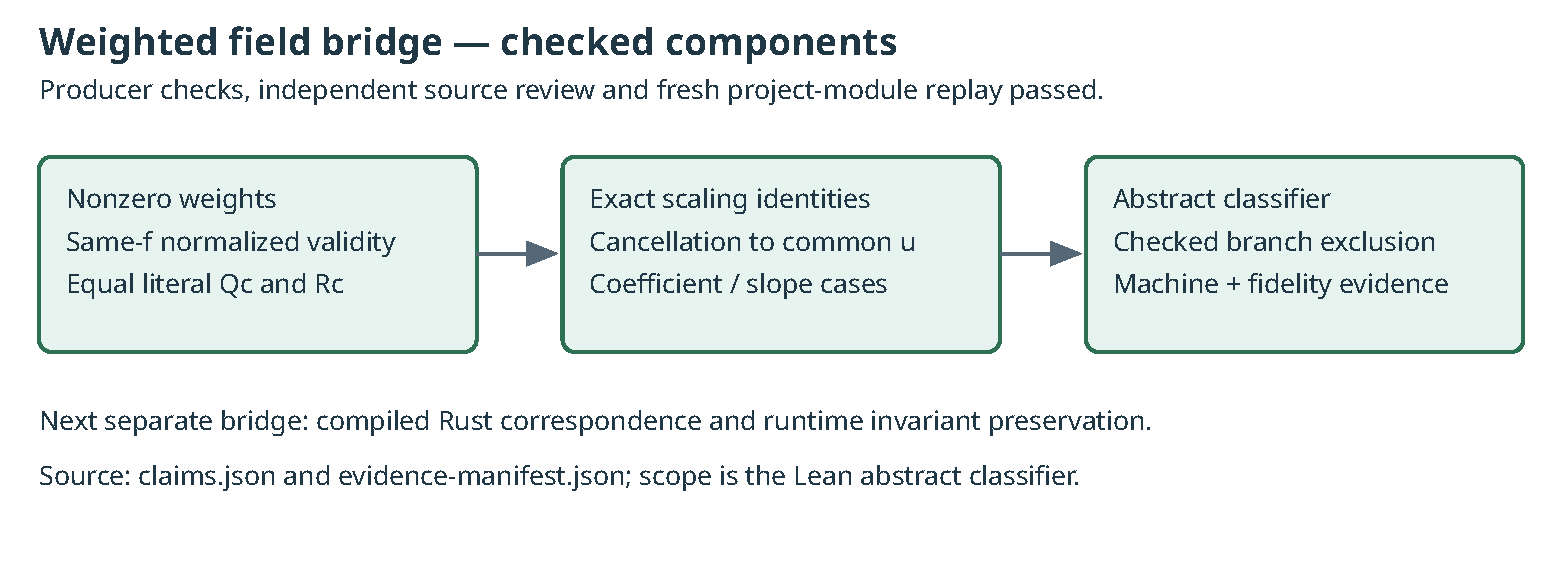
\includegraphics[width=\textwidth]{dependencies.pdf}

With $Z=z_1z_2$ and $W=w_1w_2$, nonzero-weight cancellation gives
\[
Q_{ci}=Z^2\bar q_i,\quad R_{ci}=Z^4\bar r_i,\quad
S_{ci}=Z^3W\bar s_i,\quad T_{ci}=Z^5W\bar t_i.
\]
The source proves normalized $q,r$ equality directly from cross-product equality, and normalized slope equality within the equal-$S$ case. It rewrites the second validity premise to the common support, then invokes the previously checked coefficient theorem. Its two products scale by $Z^8W^2$ and $Z^{10}W^2$ to supply the classifier helper. The unequal-$S$ case excludes the zero-slope branch directly. Inverse-before-double-before-zero-slope priority is material.

\textbf{Independent replay.} All five project modules were rebuilt from pinned sources in a fresh directory, followed by a separate declaration/axiom readback. All six processes exited zero. The inspected declarations report only \texttt{propext}, \texttt{Classical.choice}, and \texttt{Quot.sound}. Lean 4.34.1 used one thread, a 4,096 MiB limit and a 120-second external cap per compilation. The search path used the fresh directory plus the hashed dependency mirror, without producer project objects. Dependency builds were reused, not independently reproduced.

\textbf{Semantic review.} The reviewer froze a statement-only derivation and controls before receiving source, then froze the source review before compilation. The review covers the same-$f$ divisibilities, all four nonzero premises, exact powers/orientation, cancellation, and branch order. A machine replay and a source-fidelity review are separately recorded evidence streams.

\textbf{Next concrete bridge.} Connect these literal field expressions and validity premises to the compiled Rust representation and operations, including invariant preservation at calls. This theorem concerns the manually defined Lean classifier; that implementation-refinement task is separate.

\newpage
{\Large Boundary controls and operational record}

These controls are exact hand derivations in the frozen blind review, not executed experimental trials. Their complete assignments are retained in \texttt{evidence/blind-review/BLIND.md}.

\begin{tabularx}{\textwidth}{@{}p{0.29\textwidth}X@{}}\toprule
Control & Recorded observation\\\midrule
Valid unequal intercepts & Over $\mathbb Q$, weights one, $u=X^2$, $v_1=1$, $v_2=-1$, $f=1$: valid equal slopes and unequal intercepts are absorbed by the inverse branch.\\
Separate $f_1,f_2$ & Inputs $(s_1,t_1,s_2,t_2)=(1,0,1,1)$ can satisfy separate validity assertions but reach the excluded branch. Common-$f$ validity prevents this.\\
Wrong $S$ exponent & A recorded rational example changes exponent three to four, turning correct mixed slopes into equal slopes with unequal, noninverse intercepts.\\
Own instead of cross weight & A recorded rational example satisfies normalized validity but reaches the excluded branch when own weights replace opposite weights.\\
Zero weight allowed & Under Lean's totalized division, a zero-$z_1$ example satisfies normalized premises but has $S=(0,0)$ and $T=(1,0)$, reaching the excluded branch. Conventional partial division would leave the input undefined.\\
Characteristic two & No counterexample found by the stated algebraic argument: equal slopes imply equal intercepts through the square identity in characteristic two. The checked restriction is sufficient; necessity is not claimed.\\\bottomrule
\end{tabularx}

\textbf{Failures and warnings retained.} An initial independent hashing driver failed before compiler execution because \texttt{hashlib.file\_digest} was unavailable; its record and corrected driver are retained. The runtime helper emitted deprecated \texttt{if\_pos}/\texttt{if\_neg} warnings. The weighted source emitted unused/unreachable \texttt{ring} warnings. No compiler errors remained in the final independent replay. Exact command outcomes and durations are preserved in \texttt{outcomes.json} as operational records, without timing ratios.

\textbf{Packet.} This additive report preserves source, producer receipts, blind controls, source review, fresh replay outcomes, dependency/toolchain hashes and the failed-driver record. Generated Lean objects and runtime libraries are excluded. Prior reports remain unchanged. No research trial, cloud job or official ledger promotion accompanies report generation.
\end{document}
